\section{MATERIAIS E MÉTODOS}
Como já mencionado, o objetivo básico do projeto foi projetar os robôs da equipe de futebol de robôs do laboratório de robótica do DCA, sendo assim os robôs devem ter suas dimensões limitadas a um cubo de $75$mm de aresta, essa foi umas das principais restrições levada em conta para o projeto eletrônico dos robôs, além do fator econômico.  A parte estrutural do robô não será abordada neste trabalho, mas sim a parte eletrônica e de software.

\subsection{Componentes}
% Listas os componentes utilizados na montagem e mostrar algumas de suas
% principais características e sua finalidade no projeto
% mostrar o diagrama eletrônico
% Falar um pouco sobre o funcionamento dos sensores
% Falar como foi implementado a leitura, as otimizações feitas
São quatro o número de componentes básicos que compõem os robôs presentes neste trabalho, sendo eles: um par de atuadores (motor direito e esquerdo), um par de sensores de rotação (\textit{Encoder}s magnéticos), um driver motor multicanal, um microcontrolador e bateria recarregável. Devido as características dos componentes escolhidos para o projeto, apenas estes quatro tipos foram suficiente para compor a eletrônica do robô de forma a respeitar as restrições dimensionais, realizar o controle feedforward/backward de forma eficiência e com um bom período de amostragem e baixo gasto energético, além de um baixo custo financeiro.

A seguir serão apresentados mais detalhes dos componentes supracitados.

% 30:1 Micro Metal Gearmotor HP 6V with Extended Motor Shaft
\begin{figure}[H]
    \centering
    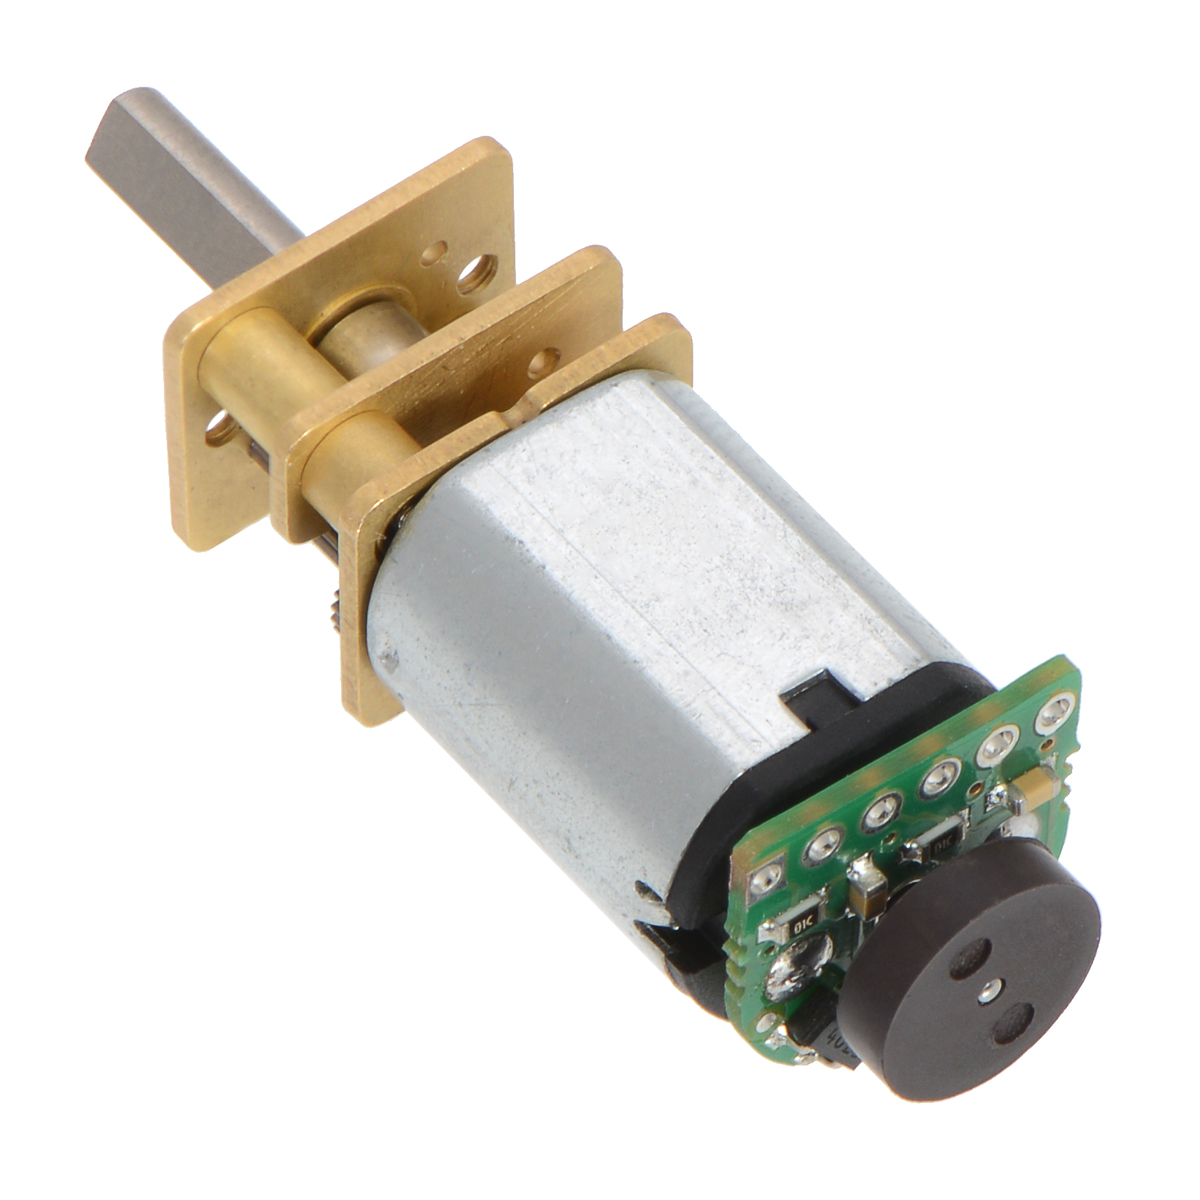
\includegraphics[width=3cm]{imagens/eletronica/motor_com_encoder.jpg}
    \caption{Micro Motor de 6V com caixa de redução de 30:1 e \textit{Encoder} magnético.}
    \label{fig:motor_com_encoder}
\end{figure}

A figura \ref{fig:motor_com_encoder} mostra o motor escolhido já com o \textit{Encoder} magnético colocado em seu eixo estendido (placa de circuito impresso com um Imã natural em forma de disco), esse é um micro motor de $6$V com uma caixa de redução de $\approx 30:1$ da \textit{Pololu}[?].

\begin{figure}[H]
    \centering
    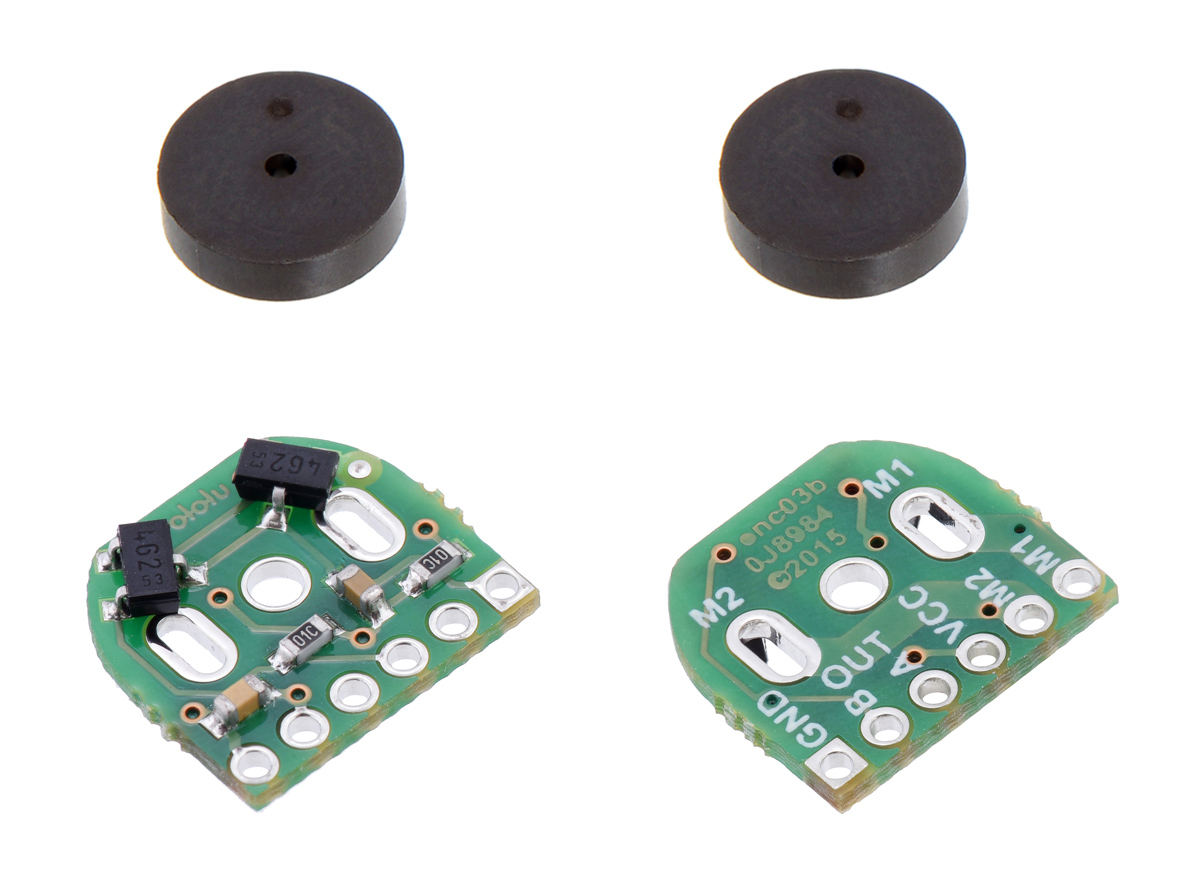
\includegraphics[width=5cm]{imagens/eletronica/encoder_frente_verso.jpg}
    \caption{Par de Encoders Magnéticos de $12$ pulsos por revolução ($12$CPR)}
    \label{fig:encoder}
\end{figure}

\begin{figure}[H]
    \centering
    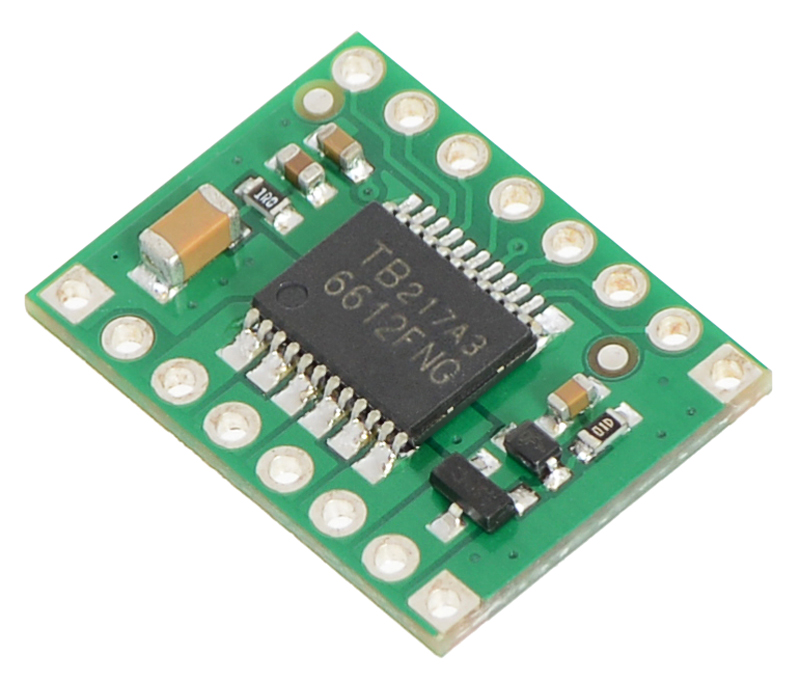
\includegraphics[width=3cm]{imagens/eletronica/driver.jpg}
    \caption{\textit{Driver} Motor TB6612FNG.}
    \label{fig:driver_motor}
\end{figure}

\begin{figure}[H]
    \centering
    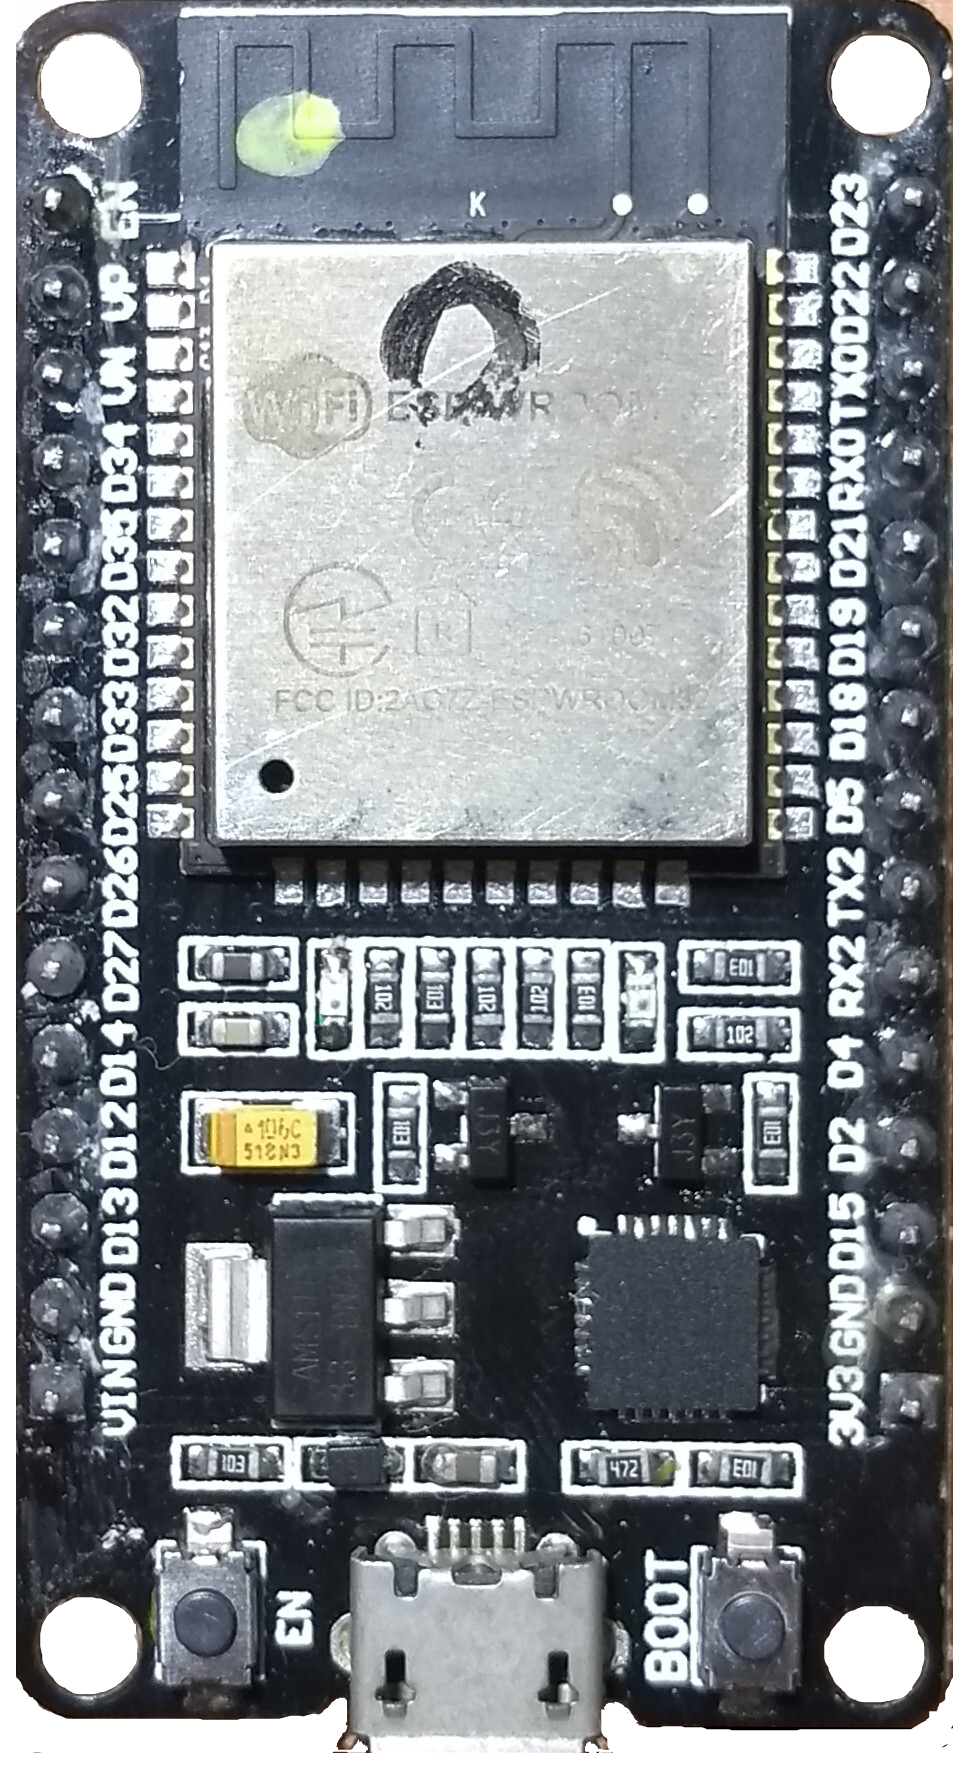
\includegraphics[width=3cm]{imagens/eletronica/esp32_kit.png}
    \caption{Placa de desenvolvimento ESP32 Dev1.}
    \label{fig:esp32_kit}
\end{figure}

\begin{figure}[H]
    \centering
    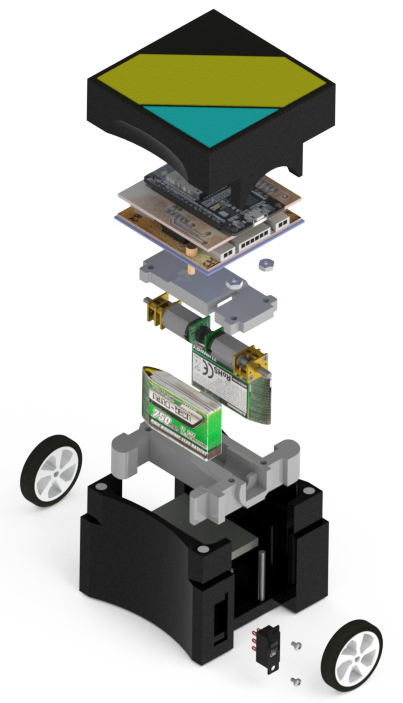
\includegraphics[width=5cm]{imagens/robo_completo_explodido.png}
    \caption{Vista explodida do robô completo.}
    \label{fig:robo_completo_explodido}
\end{figure}

\subsection{Placa de Circuito Impresso}
% CIRCUITO ELÉTRICO/ELETRÔNICO COMPLETO
% MOSTRAR/EXPLICAR: PLACA DE CIRCUITO IMPRESSO DESENVOLVIDA
% TODO:
% ref:  https://produza.ind.br/gestao/pre-requisitos-tecnicos-para-montar-um-projeto-eletronico/

% \begin{figure}[H]
%     \centering
%     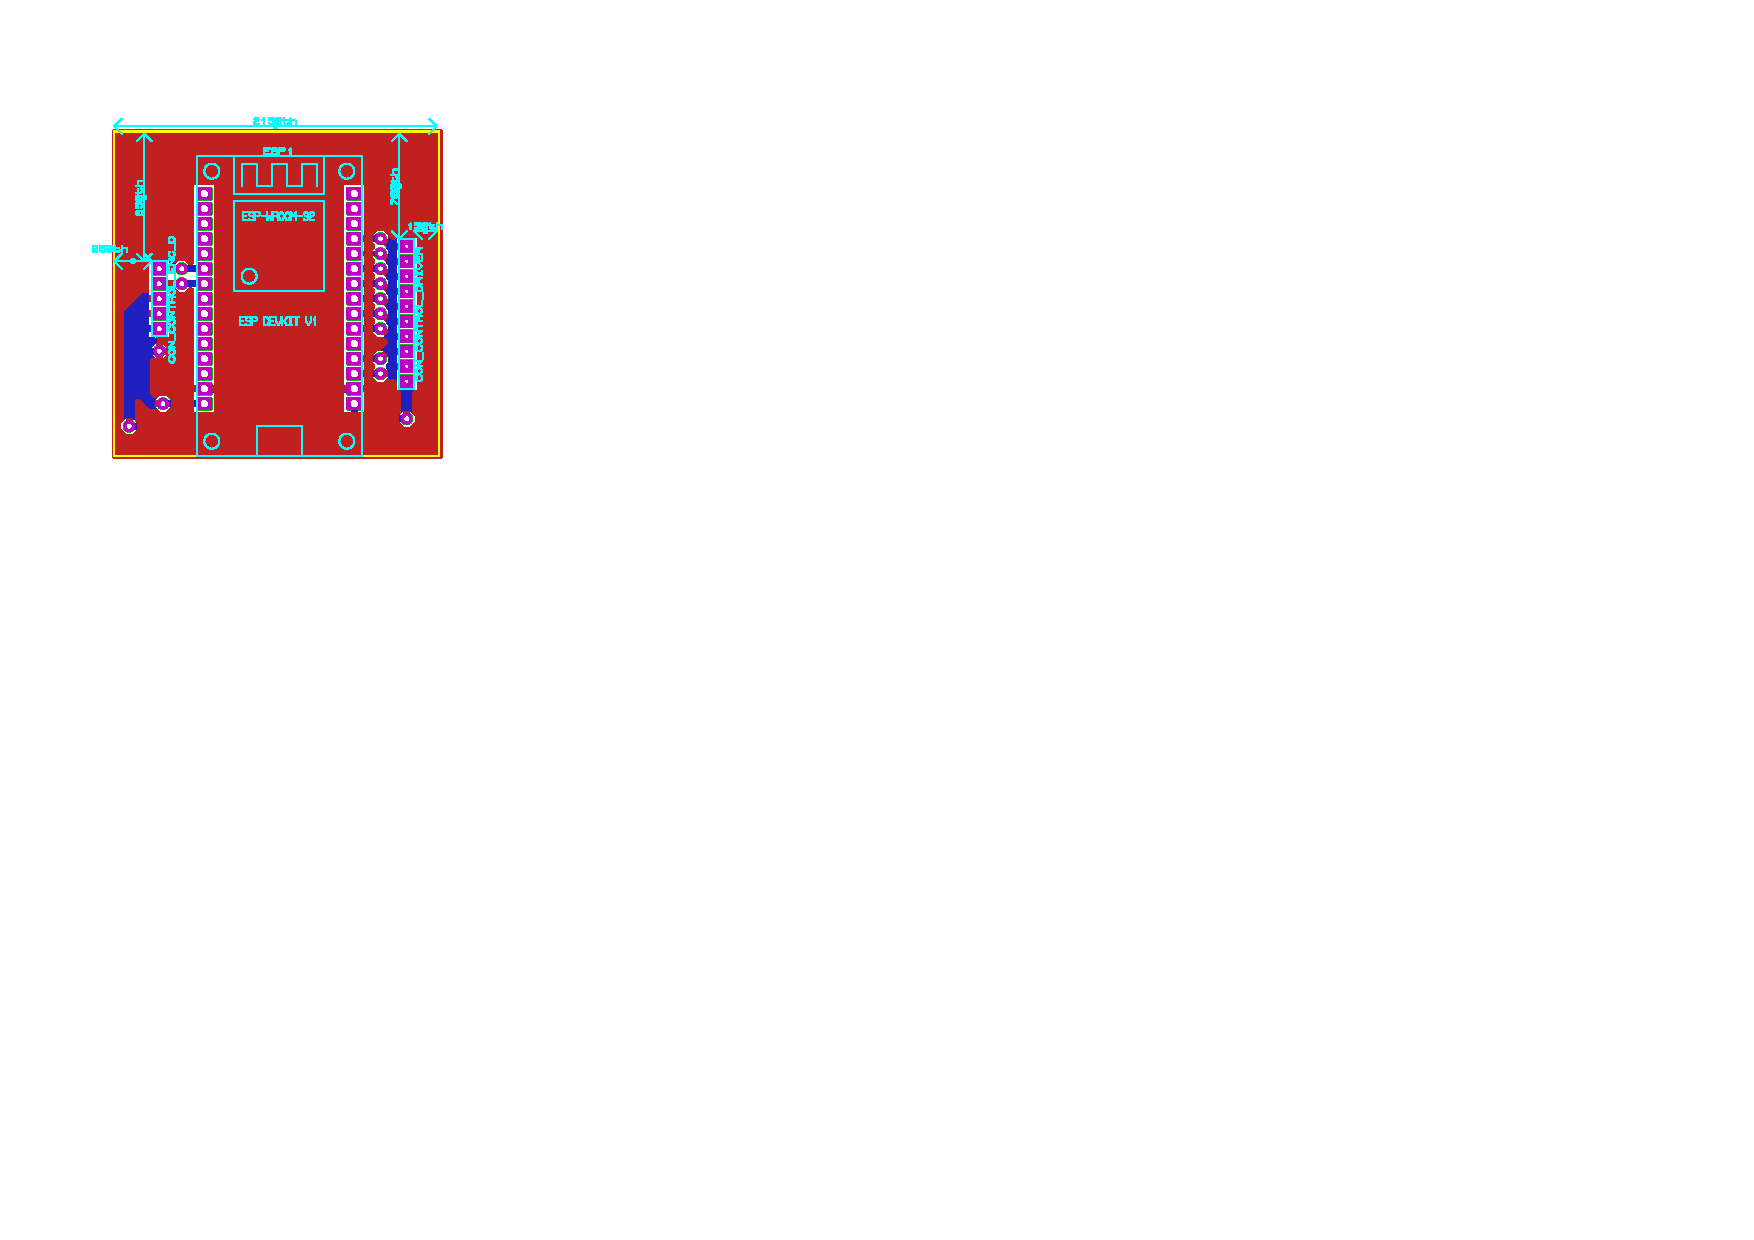
\includegraphics[width=\textwidth]{imagens/eletronica/placa/placa_controle_completa.pdf}
%     \caption{Caption}
%     % \label{fig:my_label}
% \end{figure}

% \begin{figure}[H]
%     \centering
%     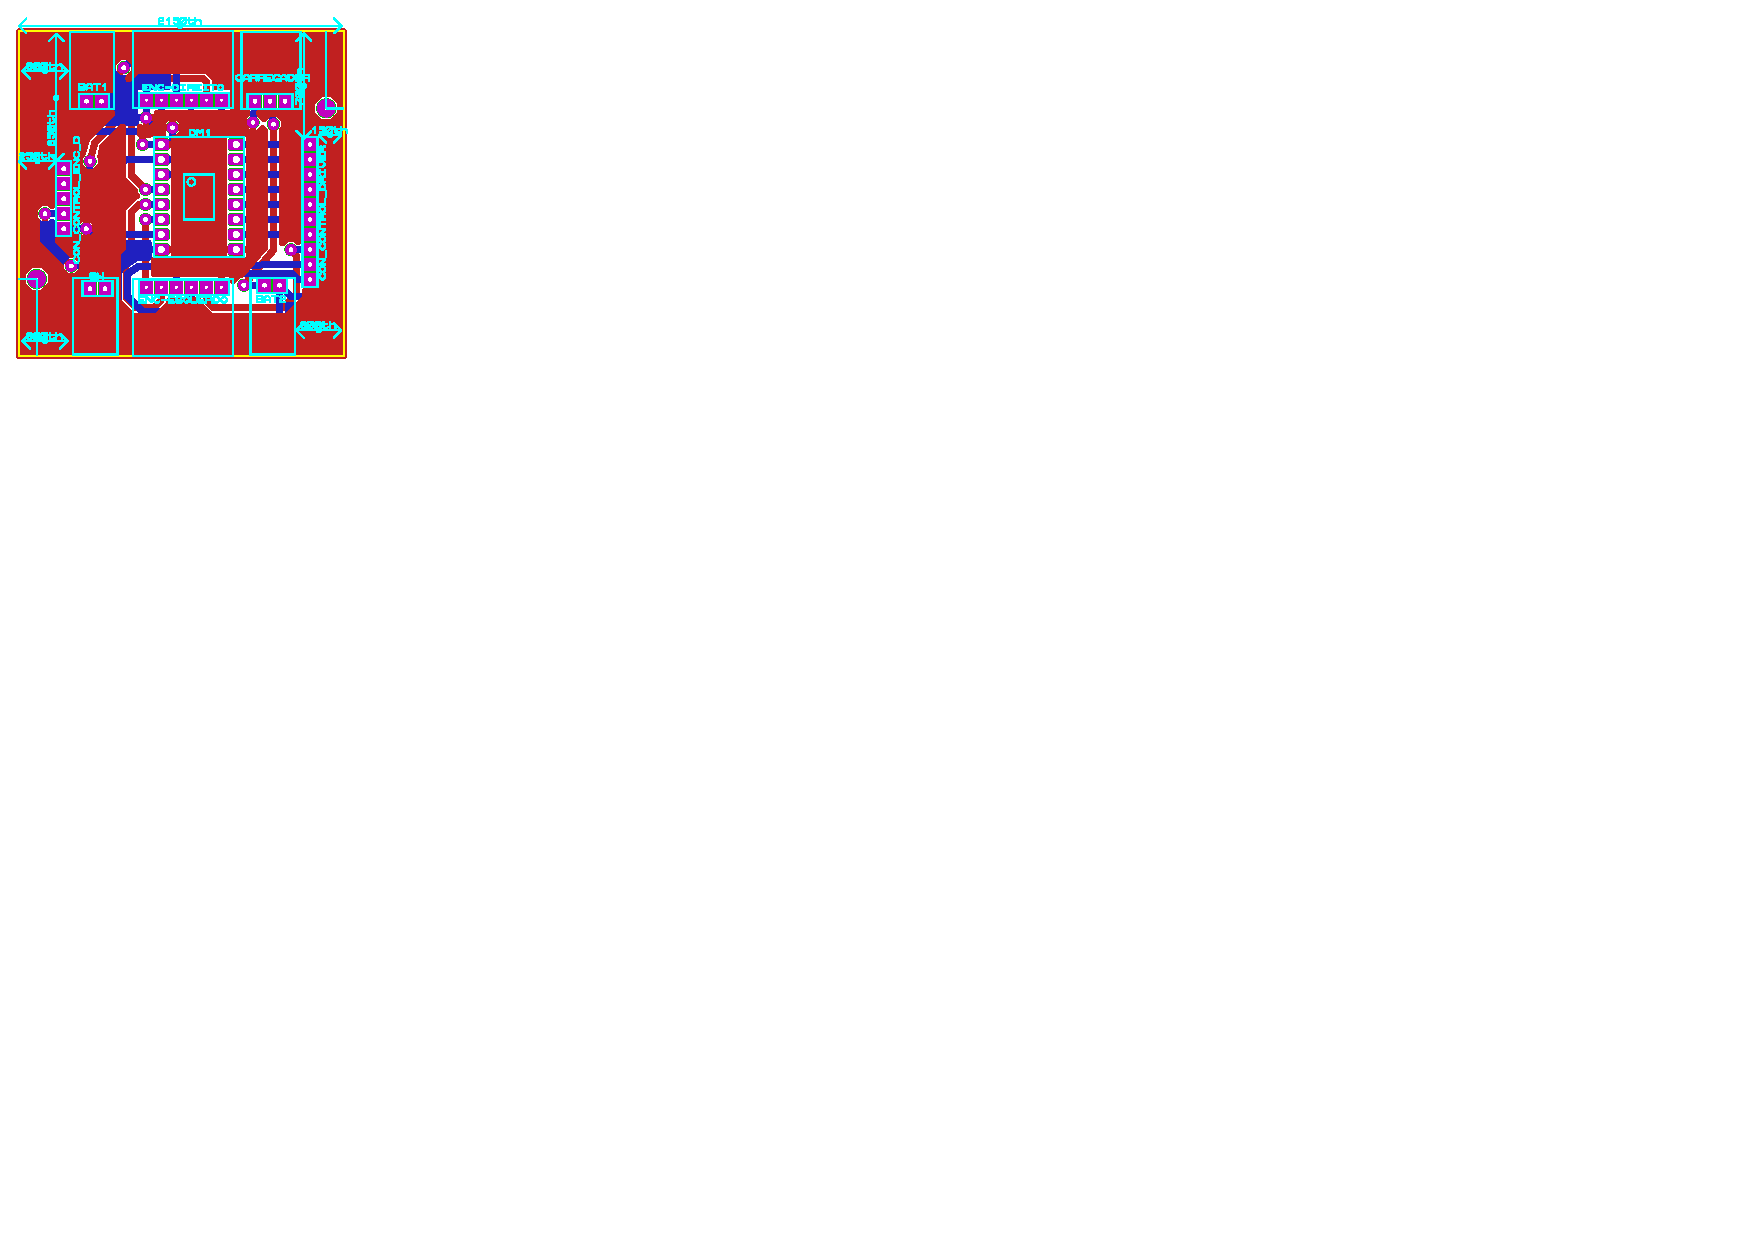
\includegraphics[width=\textwidth]{imagens/eletronica/placa/placa_driver_completa.pdf}
%     \caption{Caption}
%     % \label{fig:my_label}
% \end{figure}

\begin{enumerate}
    \item \textbf{Concepção inicial}:
        O principal objetivo por trás de se fazer uma nova placa de circuito eletrônico é acomodar os componentes, respeitando os limites das dimensões estabelecidos pela competição na qual os robôs serão utilizados (caber dentro de um cubo de $75$ mm de aresta). A placa deve conter o microcontrolador, no seu kit de desenvolvimento, \textit{Driver motor} para acionamento dos motores DCs, os \textit{Encoders} e ser alimentada por duas baterias de $1$ célula do tipo \textit{Lipo}.
        
    \item \textbf{Elaboração dos esquemáticos eletrônicos}:
        O esquemático foi a parte mais simples, pois não houve grandes mudanças nessa parte, com relação aos projetos de anos anteriores. A maior mudança foi o microcontrolador, que provocou dificuldades maiores na etapa seguinte, a elaboração do \textit{Layout}, devido às dimensões dos componentes.
        
        % inserir imagem do esquemático geral aqui
        
        \begin{figure}[H]
            \centering
            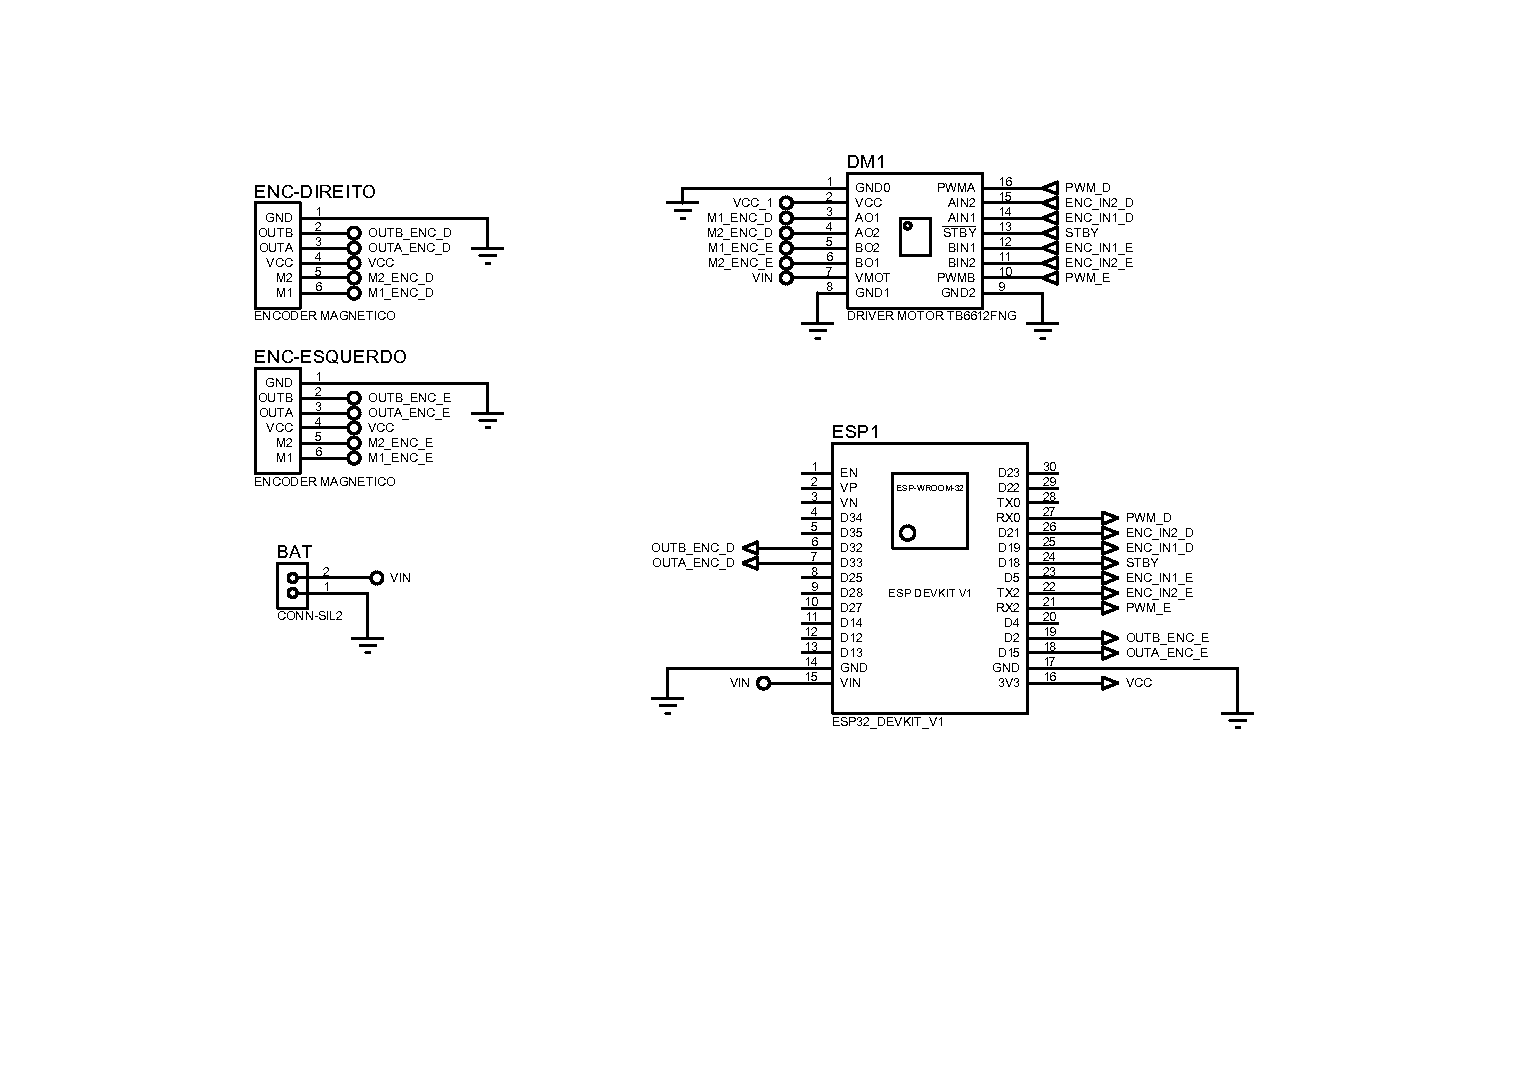
\includegraphics[width=\textwidth]{imagens/eletronica/placa/esquematico_completo.pdf}
            \caption{Esquemático.}
        \end{figure}
        
    \item \textbf{Elaboração do layout}:
        % inserir imagem do layout final aqui
        Este ponto foi o mais crítico nessa tarefa, devido à restrição de tamanho da placa ser de um quadrado com até $55$mm de lado. A solução adotada foi fazer em duas camadas, ou seja, duas placas cobreadas, ambas dupla face, dividindo os componentes. Em uma placa foi comportado o \textit{Driver}, bem como os conectores para os motores com os sensores e os conectores das baterias, e na outra apenas o microcontrolador. Para a conexão entre as placas foi utilizado um conector do tipo \textit{Head}, um macho e uma fêmea. Dessa forma, as placas conseguiram respeitar o limite dimensional e comportar todos os componentes necessários.
    \item \textbf{Realização de testes}:
        % faltou imagem de testes aqui
        Foram realizados testes antes da concepção da PCI, em \textit{Protoboards} para conferir se o circuito está funcionando como esperado e após a confecção, para se verificar a qualidade da confecção das placas.
        
        Também foram realizados testes individuais nos componentes, principalmente nos sensores, com o uso de osciloscópios. Verificou-se o funcionamento correto dos \textit{Encoders} e também conferiu-se se a distância entre os sensores poderia estar gerando interferência um no outro. Os resultados desses testes foram que todos os \textit{encoders} utilizados estão em bom estado, ou seja, funcionando como esperado e a distância que eles ficarão ao serem acomodados na estrutura não causa interferência um no outro.
    \item \textbf{Verificação e validação}
        Após testes individuais, de cada componente, foram realizados testes com a montagem completa, ou seja, os robôs montados por completo com as PCIs, baterias, motores e sensores. A validação foi por meio de controle manual dos robôs e testes simples de leitura de \textit{Encoder}, pois nessa etapa o \textit{Firmware} ainda não havida sido implementado.
\end{enumerate}

\subsection{O \emph{Firmware}}
% Falar sobre como foi feito a divisão das atividades no microcontrolador
% Mostrar ilustração dessa divisão, para ter-se uma visão global das rotinas e suas relações de dependência

\subsubsection{Rotina de Calibração}

Rotina responsável por realizar a identificação dos parâmetros do modelo dos motores direito e esquerdo do robô: constante de tempo; ganho de malha aberta; parâmetros do controlador \emph{FeedForward}; velocidade máxima de cada motor. Bem como calcular os ganhos para o controlador \emph{PID} de forma a se obter uma resposta pré-definida em malha fechada.\\

A rotina de calibração consiste em três etapas que são repetidas para todas as configurações: motor direito para frente; motor direito para trás; motor esquerdo para frente e motor esquerdo para trás. Cada etapa é descrita a seguir: 

% TO DO:
% ORGANIZAR E REPENSAR A FORMA DE EXIBIR AS ETAPAS
% FIGURAS ILUSTRANDO O COMPORTAMENTO GERAL DAS FUNÇÕES QUE ESTÃO SENDO USADAS NA INTERPOLAÇÃO
% PSEUDO CÓDIGOS TALVEZ
\begin{itemize}
    \item \textbf{ETAPA 1}: Estimar a zona morta e o ganho da planta em malha aberta\\
    
    Para isso é realizado a coleta de $N$ pontos ($\omega$,$u$), o primeiro ponto é coletado para $u = \pm1$(valor máximo no sentido de giro atual) e é realizado sucessivos decréscimos neste valor até a parada do motor ($\omega = 0$). \\
    
    Aplicar sinal de controle atual ($u_i$);\\
    Aguardar um tempo fixo, pré-determinado, para garantir a leitura de $\omega_{ss}$(velocidade de máxima/velocidade de regime)
    Armazenar ($u_i$,$\omega_{ss}$).\\
    
    A aquisição destes pontos ocorre da maior velocidade para a menor devido à zona morta ser mais baixa neste sentido, por causa da inercia do motor.\\
    
    Ao se encerrar a coleta destes pontos ($\omega_{ss} = 0$ detectado) é realizado uma regressão linear por \textit{MMQ}, tendo $\omega$ no eixo das ordenadas e $u$ no eixo das abscisas, o coeficiente angular dessa reta relaciona a velocidade angular ($\omega$) com o sinal de controle ($u$), já o coeficiente linear representa a zona morta, ou seja, o menor $u$ que pode iniciar o giro do motor.
    
    \begin{equation*}
        u(\omega) = a\omega + b
    \end{equation*}
    
    Com esses parâmetros dessa reta é possível estimar o ganho de malha aberta da planta da seguinte forma:
    
    \begin{equation*}
        K = \frac{(u_{max} - b)}{a}
    \end{equation*}
        
    \begin{figure}[H]
        \centering
        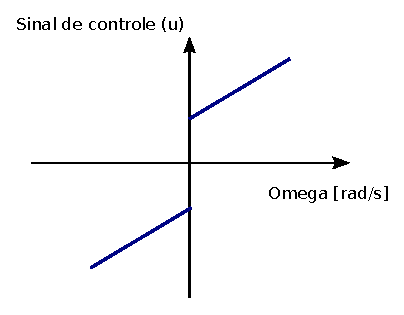
\includegraphics[width=0.5\textwidth]{imagens/ilustracoes/omega_x_sinal_controle.eps}
        \caption{Comportamento da curva $u(\omega)$.}
        \label{fig:ilustracao_omega_x_pwm}
    \end{figure}    
        
    \item \textbf{ETAPA 2}: Estimar a constante de tempo
    
    Para obter a constante de tempo da planta na configuração atual, faz-se uso mais uma vez de interpolação por \textit{MMQ} e tira-se proveito do conhecimento do ganho da planta para simplificar e tornar possível essa interpolação de forma simples. Para estimar a constante de tempo obtém-se $M$ pontos ($t$,$\omega$) e aplica-se o \textit{MMQ} para uma interpolação linear, para isso é necessário fazer a seguinte alteração:
        

    \begin{align*}
        \omega(t) &= K\left( 1 - e^{-t/T_m} \right)\\
        \ln{\omega(t)} &= \ln\left[K( 1 - e^{-t/T_m})\right]\\
        \ln\left(1 - \frac{\omega(t)}{K} \right) &= -\frac{t}{T_m}\\
        y_{aux}(t) &= -\frac{t}{T_m}
    \end{align*}
    
    Convertendo $\omega(t)$ para $y_{aux}(t)$ o coeficiente angular resultante da interpolação linear será: $coef.angular = -\frac{1}{T_m}$, dessa forma obtemos a constante de tempo.
    
    \item \textbf{ETAPA 3}: Calcular os parâmetros do controlador \textit{PID}
    
    Como apresentado na seção de referencial teórico é possível relacionar o ganho do controlador proporcional com o polo desejado para o sistema em malha fechada, por meio da relação (??). Esse cálculo só é possível devido a identificação dos parâmetros da planta resultante das etapas anteriores. O polo desejado para todas as configurações da planta é uma constante pré-definida pelo usuário.
    
\end{itemize}

Ao se passar por todas as configurações de motor/sentido a rotina seleciona a menor velocidade máxima apresentada por alguma dessas configurações e armazena esta velocidade como sendo a velocidade máxima atingida pelos motores deste robô, isso é importante, para assegurar que a referencia $\omega_{ref}$ seja factível para todas as configurações. \\

Por fim os resultados são armazenados na memória permanente do microcontrolador, sendo atualizado/sobrescrita apenas ao final da próxima chamada da rotina de calibração.

\subsubsection{Rotina de Comunicação}
% TODO:
% IDEIA: ILUSTRAR A INTERAÇÃO ENTRE A ROTINA PRINCIPAL E A INTERRUPÇÃO
A rotina de comunicação opera em um \emph{loop} infinito no núcleo principal do microcontrolador e é responsável por tratar os telecomandos recebidos pelo \textit{Bluetooth}. Ao ser identificado um recebimento de mensagem pela sinal de interrupção da comunicação \textit{Bluetooth} é acionado a função de tratamento de interrupção correspondente que possui como única função encaminhar as mensagens válida (verificar cabeçalho) para a rotina principal de comunicação. Isso é feito para evitar sobrecarregar a interrupção, já que ela deve operar em altas frequências.\\

Na rotina principal a mensagem é interpretada e caso ela seja identificado um telecomando válido, será executado a devida resposta, conforme apresentado a seguir.

O protocolo implementado, foi pensado para conter até três grandes campos, o \textbf{\textit{Head}} com 4 bits de preambulo, para ajudar a sincronizar os pacotes, o \textbf{\textit{Cmd}} também com 4 bits, possibilitando assim até 16 comandos distintos e o campos de argumentos com tamanho variável. Foram implementados 7 comandos. 

% Please add the following required packages to your document preamble:
% \usepackage[table,xcdraw]{xcolor}
% If you use beamer only pass "xcolor=table" option, i.e. \documentclass[xcolor=table]{beamer}
\begin{table}[H]
\centering
\begin{tabular}{c|r}
\hline
\rowcolor[HTML]{C0C0C0} 
\multicolumn{1}{|c|}{\cellcolor[HTML]{C0C0C0}DEFINIÇÕES} & \multicolumn{1}{r|}{\cellcolor[HTML]{C0C0C0}VALOR(HEX)} \\ \hline
HEAD & A0 \\
\rowcolor[HTML]{EFEFEF} 
CMD\_REQ\_CAL & 00 \\
CMD\_REQ\_OMEGA & 03 \\
\rowcolor[HTML]{EFEFEF} 
CMD\_CALIBRATION & 04 \\
CMD\_IDENTIFY & 05 \\
\rowcolor[HTML]{EFEFEF} 
CMD\_SET\_POINT & 0A \\
CMD\_CONTROL\_SIGNAL & 0B \\
\rowcolor[HTML]{EFEFEF} 
CMD\_PING & 0F
\end{tabular}
\caption{Definições utilizadas.}
\label{tab:my-table}
\end{table}
    
\textbf{Comandos}
\begin{itemize}
    \item \textbf{CMD\_REQ\_CAL}:\\
        \textit{Host} envia, para solicitar os dados provenientes da calibração do controlador \textit{feedforward}. O escravo (robô) envia 4 \emph{floats}, referente aos coeficientes do controlador.
    \item \textbf{CMD\_REQ\_OMEGA}:\\
        \textit{Host} envia, para solicitar as velocidades atuais de ambos os motores, em $rad/s$. O escravo responde com dois \emph{floats}, referentes aos ômegas em cada motor.
    \item \textbf{CMD\_CALIBRATION}:\\
        \textit{Host} envia, para fazer com que o robô inicie sua rotina de calibração do controlador.
    \item \textbf{CMD\_IDENTIFY}:\\
        \textit{Host} envia, fazendo com que o robô inicia sua rotina de identificação. O \textit{Host} deve enviar o \emph{bitstream} da seguinte forma:\\
        
        % Please add the following required packages to your document preamble:
% \usepackage{graphicx}
% \usepackage[table,xcdraw]{xcolor}
% If you use beamer only pass "xcolor=table" option, i.e. \documentclass[xcolor=table]{beamer}
\begin{table}[H]
\centering
\resizebox{\textwidth}{!}{%
\begin{tabular}{|
>{\columncolor[HTML]{C0C0C0}}l |
>{\columncolor[HTML]{C0C0C0}}l |l|l|l|}
\hline
HEAD & CMD\_IDENTIFY & OPTIONS & SETPOINT & STEPTIME \\ \hline
\end{tabular}%
}
\end{table}
        
        Sendo o campos \textbf{options} de 1 byte, contendo a informação de qual motor será feita a identificação e se deve ser usado o controlador.
        
        Ao concluir a rotina de identificação, o robô responde enviando o vetor de ômegas medidos, durante a rotina, para o \textit{host}, que deve estar aguardando recebê-las. A quantidade de dados será $\frac{timeout}{steptime}*4$ bytes, portando o \textit{host} deve estar aguardando exatamente essa quantidade de bytes.
        
        
    \item \textbf{CMD\_SET\_POINT}:\\
        
        % Please add the following required packages to your document preamble:
% \usepackage{graphicx}
% \usepackage[table,xcdraw]{xcolor}
% If you use beamer only pass "xcolor=table" option, i.e. \documentclass[xcolor=table]{beamer}
\begin{table}[H]
\centering
\resizebox{\textwidth}{!}{%
\begin{tabular}{|
>{\columncolor[HTML]{C0C0C0}}c |
>{\columncolor[HTML]{C0C0C0}}c |c|c|c|c|l|l|l|}
\hline
HEAD & CMD\_SET\_POINT & SENSE\_L & OMEGA\_L & SENSE\_R & \multicolumn{4}{c|}{OMEGA\_R} \\ \hline
\end{tabular}%
}

\end{table}
        
        Neste os campos de \textbf{sense\_x} indicam o sentido de rotação do motor, 0 para trás e 1 para rodar para frente (convertidos em sinal dos ômegas de setpoint), portando só ocupam 1 bit, já os campos referentes aos ômegas desejados ocupam 15 bits, sendo assim é possível enviar referências com uma precisão de $1.0/2^{15}$, já que as referências serão enviadas inteiras  (0 - $2^{15}$) e mapeadas de $-1.0$ a $1.0$, indicando uma porcentagem da referência da velocidade máxima do robô. Ou seja os campos referentes aos \textit{setpoints} contêm a porcentagem da velocidade máxima do robô.
        
    \item \textbf{CMD\_CONTROL\_SIGNAL}:\\
        
        O comando difere apenas o campo de \textbf{cmd} do comando anterior. O restante da estrutura é exatamente igual, pois a principal diferença ocorre no microcontrolador. Em vez dos campos referentes aos ômegas serem porcentagens da velocidade máxima que será convertido em \textit{Setpoint} para o controlador, neste comando o robô irá interpretar esses campos como sendo sinais de controle (após convertê-los para \emph{float} de $-1.0$ a $1.0$).
        
    \item \textbf{CMD\_PING}:\\
        Neste comando o \textit{host} pode enviar qualquer mensagem no campo de argumentos, pois o robô irá apenas responder com a mesma mensagem. Este comando é útil para testar conexão e testar a latência da conexão.
    
\end{itemize}

% TABELA TEMPORÁRIA
\begin{table}[H]
\resizebox{\textwidth}{!}{
\begin{tabular}{|l|c|c|l|}
\hline
\multicolumn{1}{|c|}{Command Tag} & \multicolumn{1}{l|}{Hex} & Arg. & \multicolumn{1}{c|}{Description} \\ \hline
CMD\_REQ\_CAL & 0x00 & - & \begin{tabular}[c]{@{}l@{}}Solicita ao microcontrolador que envie os\\ dados da última calibração, que estão armazenados na memória flash.\end{tabular} \\ \hline
 &  &  &  \\ \hline
 &  &  &  \\ \hline
CMD\_REQ\_OMEGA & 0x03 & - & \begin{tabular}[c]{@{}l@{}}Solicita ao microcontrolador que envie as leituras atuais da velocidade\\ de rotação, em rad/s, dos dois motores. O microcontrolador enviará dois\\ floats, sendo primeiro float refererente ao motor esquerdo e o segundo ao\\ motor direito.\end{tabular} \\ \hline
CMD\_CALIBRATION & 0x04 & - & \begin{tabular}[c]{@{}l@{}}Sinaliza para o microcontrolador que ele deve iniciar a rotina de calibração\\ dos parâmetros do controlador, bem como os parâmetros para o filtro de Kalman.\end{tabular} \\ \hline
CMD\_IDENTIFY & 0x05 & - & \begin{tabular}[c]{@{}l@{}}Sinaliza para o microcontrolador que ele deve iniciar a rotina \\ de coleta dos dados  de identificação e ao final deve enviar \\ esses dados para o host.\end{tabular} \\ \hline
 &  &  &  \\ \hline
 &  &  &  \\ \hline
 &  &  &  \\ \hline
 &  &  &  \\ \hline
CMD\_REF & 0x0A & \begin{tabular}[c]{@{}c@{}}ref. Left (15bits)\\ ref.Right (15 bits)\end{tabular} & \begin{tabular}[c]{@{}l@{}}Informa ao microcontrolador qual referência aplicar para \\ o controlador de velocidade de rotação. \\ As referências estão no intervalo {[}-1.0, 1.0{]}.\end{tabular} \\ \hline
CMD\_CONTROL\_SIGNAL & 0x0B & \begin{tabular}[c]{@{}c@{}}pwm. Left (15bits)\\ pwm.Right (15 bits)\end{tabular} & \begin{tabular}[c]{@{}l@{}}Informa ao microcontrolador qual sinal de controle aplicar. \\ Valores no intervalo {[}-1.0, 1.0{]}.\end{tabular} \\ \hline
 &  &  &  \\ \hline
 &  &  &  \\ \hline
CMD\_RESET & 0x0E &  &  \\ \hline
CMD\_PING & 0x0F & mensagem qualquer & Sinaliza para o microcontrolador que ele deve apenas devolver a mensagem para o host. \\ \hline
\end{tabular}
}
\caption{}
\label{tab:command_table}
\end{table}

\subsubsection{Rotina de Controle}
% TODO:
O controle é executado sozinho no núcleo secundário do ESP32 em \emph{loop} infinito com uma taxa de atualização de $5ms$. A rotina consiste em receber as velocidades providas pela de leitura dos sensores por meio de mensagens entre processos, em seguida é realizado a etapa de controle propriamente dita, que consiste em aplicar a ação do controle \textit{FeedForward} somado a ação do controle de malha fechada, tendo como entrada a última referência de percentual de velocidade lida pela rotina de comunicação multiplicada pela velocidade máxima considerada para a rotação do eixo do motor, para passar a referência para $rad/s$. \\

Ao final do fluxo de controle tem-se o sinal de controle, este por sua vez é utilizado para configurar o sentido de giro e o sinal \emph{PWM} que deve ser aplicado no \emph{Driver} motor correspondente.

\subsubsection{Rotina de Leitura dos Sensores}
% TODO:
% REALIZAR ANÁLISE DE FREQ. MÁXIMA DE OPERAÇÃO DOS ENCODERS VS BANDA DISPONIVEL NAS INTERRUPÇÕES RESPONSAVEIS PELA LEITURA DOS ENCODERS

Há duas interrupções associadas aos sinais provenientes dos \emph{Encoders} rotativos, uma para cada motor, cujo objetivo é calcular/medir a velocidade de rotação do eixo do motor ($\omega_{medido}$) bem como aplicar o filtro de \emph{Kalman} para uma melhor estimativa da mesma. As interrupções são provocadas pelas bordas dos pulsos de ambos os canais, fazendo com que a resolução do sensor seja utilizada ao máximo, pois dessa maneira os sensores que possuem uma resolução de três pulsos completos por revolução (em cada canal, ver Figura \ref{fig:ilustracao_uma_revolucao}) consegue acionar doze ($12$) vezes a interrupção que irá computar o $\omega_{motor}$, passando assim a ser ter uma resolução de doze pulsos por revolução.\\

Para o cálculo do módulo da velocidade de rotação do eixo do motor faz-se:
\begin{equation}
    |\omega_{medido}| = \frac{2\pi}{NPR}\frac{1}{\Delta{t}}
    \label{eq:modulo_omega_medido}
\end{equation}

Onde $NPR$ é o número pulsos por revolução em um canal. Neste trabalho o $NPR$ é igual a três($3$). Já o intervalo $\Delta{t}$ é o intervalo entre bordas iguais em um canal, a Figura \ref{fig:sinal_em_quadratura_delta_t} ilustra esse intervalo para as bordas de subida de ambos os canais.\\

\begin{figure}[H]
    \centering
    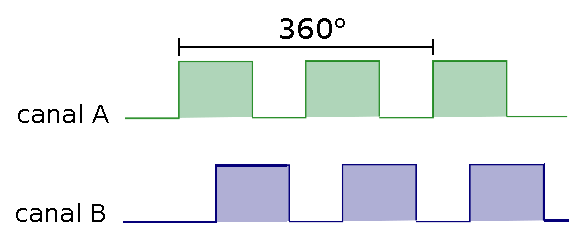
\includegraphics[width=0.5\textwidth]{imagens/ilustracoes/sinal_enquadratura_uma_revolucao.eps}
    \caption{Ilustração do sinal em quadratura em uma revolução completa do eixo do motor no sentido horário.}
    \label{fig:ilustracao_uma_revolucao}
\end{figure}

\begin{figure}[H]
    \centering
    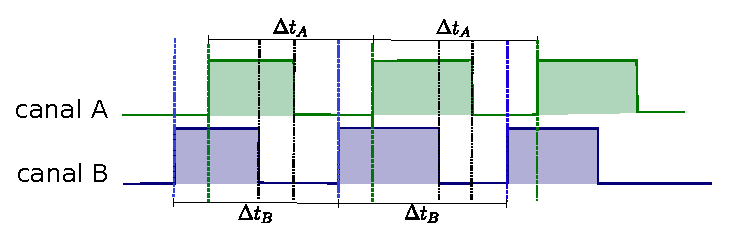
\includegraphics[width=0.6\textwidth]{imagens/ilustracoes/sinal_em_quadratura_sentido_CCW_detalhada.eps}
    \caption{Ilustração de um sinal em quadratura para uma revolução do eixo do motor sentido anti-horário para um \emph{Encoder} com a resolução de três pulsos por revolução, com destaque para o intervalo de tempo entre as bordas de subida de um mesmo canal.}
    \label{fig:sinal_em_quadratura_delta_t}
\end{figure}

% Please add the following required packages to your document preamble:
% \usepackage{graphicx}
\begin{table}[H]
\centering
\resizebox{0.5\textwidth}{!}{%
\begin{tabular}{cc|cc}
\multicolumn{2}{c|}{\textbf{\begin{tabular}[c]{@{}c@{}}Sentido\\     Horário\end{tabular}}} &
  \multicolumn{2}{c}{\textbf{\begin{tabular}[c]{@{}c@{}}Sentido\\ Anti-Horário\end{tabular}}} \\ \hline
\textbf{A} & \textbf{B} & \textbf{A} & \textbf{B} \\
1          & 0          & 1          & 0          \\
0          & 1          & 0          & 1         
\end{tabular}%
}
\caption{Código de 2 bits para identificar o sentido de rotação.}
\label{tab:tabela_simple_code}
\end{table}

Já para se obter o sentido de rotação do motor, faz-se uso do padrão \emph{Gray Code} gerado pela diferença de fase entre os diferentes canais de um mesmo sensor, uma maneira de fazer isso é ler os \emph{GPIO}'s associados aos canais do \emph{Encoder} e verificar o padrão em binário e inferir o sentido de rotação, a Figura \ref{fig:cw_signal} ilustrado isso para uma rotação no sentido horário e a Figura \ref{fig:ccw_signal} o anti-horário, esses códigos são apresentados na Tabela \ref{tab:tabela_simple_code}. Porém esse procedimento apresentou ser pouco eficiente em medias e altas rotações, devido a alta taxa de erro na inferência do sentido. \\


A abordagem adotada aqui foi armazenar os dois \emph{bits}(sendo canal A bit mais significado) e concatenar/somar com os últimos dois \emph{bits} (da leitura anterior) deslocados em dois (equivalente à multiplicar por $2^2$ ou operar bit-a-bit: $bits_{anteriores} \ll 2$), criando assim um padrão com $4$ \emph{bits}, sendo os dois mais significados o padrão da leitura anterior e os dois menos significativos a leitura atual. Esse procedimento é ilustrado para uma rotação no sentido horário e no sentido anti-horário respectivamente nas Tabelas \ref{tab:tabela_gray_code_cw} e \ref{tab:tabela_gray_code_ccw}, dessa forma gera-se quatro($4$) padrões/códigos que caracterizam um tipo de rotação. Esse padrão de $4$\emph{bits} é armazenado de forma estática em um vetor(uma tabela de cola/ \emph{lookup table}) nas rotinas de ambos os motores, esse vetor mapeia o código binário em $1$, $-1$ ou zero para as combinações que não caracterizam um sentido de giro, o sinal do valor corresponde ao sentido horário ou anti-horário e depende do motor, um exemplo de \emph{lookup table} é apresentado na Tabela \ref{tab:lookup_table}.

\begin{figure}[H]
    \centering
    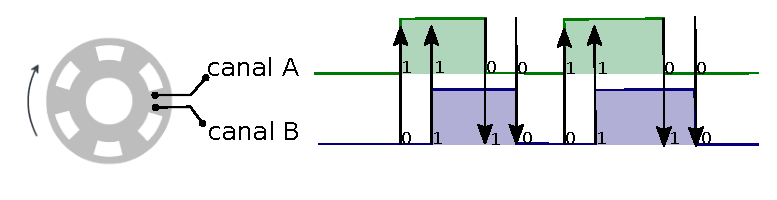
\includegraphics[width=0.7\textwidth]{imagens/ilustracoes/sinal_enquadratura_sentido_CW.eps}
    \caption{Sinal em quadratura para rotação no sentido horário.}
    \label{fig:cw_signal}
\end{figure}

% Please add the following required packages to your document preamble:
% \usepackage{graphicx}
\begin{table}[H]
\centering
\resizebox{0.5\textwidth}{!}{%
\begin{tabular}{c|c|c|c|c}
\textbf{$A_{ant}$} & \textbf{$B_{ant}$} & \textbf{$A_{atual}$} & \textbf{$B_{atual}$} & \textbf{DEC} \\ \hline
0 & 0 & 1 & 0 & 2 \\
1 & 0 & 1 & 1 & 11 \\
1 & 1 & 0 & 1 & 13 \\
0 & 1 & 0 & 0 & 4
\end{tabular}%
}
\caption{Gray Code para a rotação no sentido horário.}
\label{tab:tabela_gray_code_cw}
\end{table}

\begin{figure}[H]
    \centering
    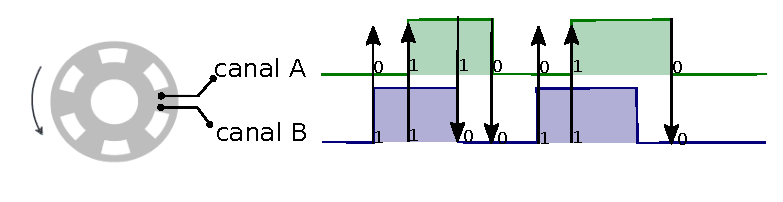
\includegraphics[width=0.7\textwidth]{imagens/ilustracoes/sinal_enquadratura_sentido_CCW.eps}
    \caption{Sinal em quadratura para rotação no sentido anti-horário.}
    \label{fig:ccw_signal}
\end{figure}

% Please add the following required packages to your document preamble:
% \usepackage{graphicx}
\begin{table}[H]
\centering
\resizebox{0.5\textwidth}{!}{%
\begin{tabular}{c|c|c|c|c}
\textbf{$A_{ant}$} & \textbf{$B_{ant}$} & \textbf{$A_{atual}$} & \textbf{$B_{atual}$} & \textbf{DEC} \\ \hline
0 & 0 & 0 & 1 & 1  \\
0 & 1 & 1 & 1 & 7  \\
1 & 1 & 1 & 0 & 14 \\
1 & 0 & 0 & 0 & 8 
\end{tabular}%
}
\caption{Codificação de 4 \emph{bits} para a rotação no sentido anti-horário.}
\label{tab:tabela_gray_code_ccw}
\end{table}

% Please add the following required packages to your document preamble:
% \usepackage{graphicx}
\begin{table}[H]
\centering
\resizebox{0.8\textwidth}{!}{%
\begin{tabular}{c|ccccllllllllllll}
\textbf{Índice} & 0 & 1  & 2 & 3 & 4 & 5 & 6 & 7  & 8  & 9 & 10 & 11 & 12 & 13 & 14 & 15 \\ \hline
\textbf{Valor}  & 0 & -1 & 1 & 0 & 1 & 0 & 0 & -1 & -1 & 0 & 0  & 1  & 0  & 1  & -1 & 0 
\end{tabular}%
}
\caption{Lookup table.}
\label{tab:lookup_table}
\end{table}

Com a \emph{lookup table} e o módulo da velocidade é possível calcular a velocidade de rotação da seguinte forma:

\begin{equation}
    \omega_{medido} = \frac{2\pi}{NPR}\frac{table[code]}{\Delta{t}}
\end{equation}

A próxima etapa é a filtragem dessa velocidade, a rotina aplica o filtro de \emph{Kalman} (mais detalhes na seção de referencial teórico) considerando $omega(t)$ um sistema de primeira ordem, como apresentado na seção sobre modelagem de motores de corrente contínua essa pode ser uma boa aproximação se desconsiderar a influência da indutância interna do motor, isso faz com as variáveis do filtro sejam modeladas para:


\begin{equation*}
\begin{cases}
    \textbf{x}_k = \left[ \omega_k \right]\\
    z_k = x_k = \omega_k\\
    F_k = 1\\
    H_k = 1
\end{cases}
\end{equation*}

Modelo da \textbf{medição}:
\begin{align*}
z_k = \omega_{medido}
\end{align*}

Com isso a etapa de \textbf{predição} do filtro torna-se:
% MUDAR O SIMBOLO QUE FAZ REFERENCIA À ENTRADA (u) DE ENTRADA
\begin{align*}
    \check{\omega}_k &= \hat{\omega}_{k-1} + u_k\left( 1 - e^{-\Delta{t}/T_m} \right)\\
    \check{P}_k &= \hat{P}_{k-1} + Q_k
\end{align*}

Sendo $u_k$ a entrada no instante $k$, $\Delta t = t_f - t_0$. $\Delta t$ é relativo ao sinal de entrada $u_k$, sendo $t_0$ o instante que o sinal é aplicado e $t_f$ o instante atual $k$.


E a etapa de atualização \textbf{Atualização} é:

\begin{align*}
K_k &= \check{P}_k \left( \check{P}_k + R_k \right)^{-1} = \frac{\check{P}_k}{\check{P}_k + R_k}\\
\hat{\omega}_k &= \check{\omega}_k + K_k \left( \omega_{k_{medido}} - \check{\omega}_k \right)\\
\hat{P}_k &= \left( 1 - K_k \right) \check{P}_k
\end{align*}


% colocar aqui pseudo código da rotina completa

% \begin{algorithm}
% \caption{A Hough Transform for Squares Detection}
% \label{alg:hough_for_squares}
% \begin{algorithmic}[1]
% \State initialize $M$ with zero. \Comment{Voting matrix initialized with zero.}
% \ForAll{$(x',y')$ in $f(x,y)$}
%     \If{$|\nabla{f(x',y')}| \geq $ edge threshold } \Comment{It's an edge.}
        
%         \State $p_0 \gets (x',y')$
%         \State $\theta \gets \angle{\nabla{f(x',y')}} \mod{90^\circ}$ \Comment{Square's angle.}
%         \State $\Vec{N_0} \gets \nabla{f(x',y')}/|\nabla{f(x',y')}|$
%         \State $\Vec{N_1} \gets -\nabla{f(x',y')}/|\nabla{f(x',y')}|$
%         \State $\Vec{N_2} \gets$ rotate $\Vec{N_1}$ on $90^\circ$\\
        
        
%         \State Search for an edge point going in the direction of $\Vec{N_1}$ from $p_0$. \Comment{That will be the $p_1$ point.}\\
        
%         \State $l \gets |p_0 - p_1|$ \Comment{Square's size.}
        
%         \State $p_{middle} \gets (p_1 + p_0)/2$\\
        
%         \State Search for an edge point going in the direction of $\Vec{N_2}$ from $p_{middle}$. \Comment{That will be the $p_2$ point.}\\
        
%         \State $p_{center} \gets p_2 - \Vec{N_2}*l/2$ \Comment{$p_{center} = (x_c,y_c)$}
        
%         \State $M[x_c][y_c][l][\theta] \gets M[x_c][y_c][l][\theta] + 1$
        
%     \EndIf
% \EndFor
% \end{algorithmic}
% \end{algorithm}


% \subsubsection{Rotina de Telemetria}
% TODO:
% NOTA:
% Não sei se seria interessante falar dessa. Ao ser ativada ela inicia o armazenamento de vários dados, como velocidades, setpoint, velocidade filtrada, velocidade não filtrada, variáveis do filtro... grava esses dados durante x segundos e ao final envia tudo ao host via bluetooth